\chapter{Discussion}
\label{ch_discussion}









% ------------------------------------------------------------------
\section{Dust Properties from Scattering Models}
% ------------------------------------------------------------------
%\subsection{Polarization Morphology}
The dominant azimuthal polarization morphology observed at \bfour suggests that the polarization from aligned dust grains has a greater contribution at longer wavelengths. However, the small minor-axis-aligned region at the centre of the disk indicates that dust self-scattering may also contribute to the polarized emission. A combination of azimuthal and uniform morphologies was observed at \bfiveNS, \bsixNS, and \bseven as well. This suggests that the polarization morphology at each wavelength may be caused by a combination of multiple polarization mechanisms, rather than from a single mechanism.


The relative size of the azimuthal and minor-axis-aligned morphologies changes with wavelength. The azimuthal morphology is more confined to the outer disk as wavelength decreases, and the minor-axis-aligned morphology becomes larger in the centre. A potential explanation for this is the change in optical depth across the disk. The optical depth of the emission increases at shorter wavelengths, and dust self-scattering should dominate at higher optical depths \citep{Williams, Lin2022}. The central region of the disk is expected to have a higher optical depth compared to the outer disk \citep{Williams}, which could favour a higher contribution from dust self-scattering and explain the increasing minor-axis-aligned region at shorter wavelengths. 

The spatial dependence of the two morphologies also suggests that the contribution from each mechanism varies across the disk. At each wavelength, the minor-axis-aligned region is most prominent at the centre, while the azimuthal morphology is most prominent towards the outer regions of the disk. Therefore, the optically thick inner disk may favour dust self-scattering, and is less favoured in the optically thin outer disk, allowing the polarization from aligned grains to have a larger contribution.






% --------------------------------------------------------------------
\section{Comparison to HL Tau}
% -------------------------------------------------------------------


\subsection{Morphology}

% They are very similar and Main differences 
The morphologies of IRS~63 (Figure \ref{fig: StokesI_POLI_grid}) and HL Tau (Figure \ref{fig: HLTauLin2024}) show a striking similarity between the morphologies in both of these disks. Both are azimuthally dominated at long wavelengths and uniformly dominated at shorter wavelengths. However, the morphologies are not exact. In IRS~63, even at the longest wavelength of \bfourNS, there is still a uniform component at the very centre of the disk, while HL Tau only shows azimuthal polarization at \bfourNS, which is depolarized at the centre. Similarly, at \bsevenNS, IRS~63 shows some azimuthal vectors on the outer edge of the disk, while the vectors for HL Tau are entirely uniform. 


The broad similarities in polarization morphology in both HL Tau and IRS 63 suggest that a wavelength-dependent change in polarization morphology is not unique to either disk, and may be caused by the same changes in the contribution of the polarization mechanisms with wavelength. Additionally, the difference in the spatial dependence suggests that there is something else in these disks contributing to this difference. In the following subsections, we discuss potential differences between the two disks.


% --------------------------------------------------------------------
\subsection{Evolutionary Stage and Structure}
% --------------------------------------------------------------------
%%%%%%%%%%%% EVOLUTIONARY STAGE and SUBSTRUCTURE %%%
% As a separate paragraph, I suggest you comment on evolutionary stage and substructure.

% Specifically, HL Tau has a series of rings and gaps (can reference the initial HL Tau image that shows all the rings from early ALMA days) and IRS 63 is also structured (reference Dom).  Stephens et al. (2023) made a high-resolution polarization study of HL Tau, showing that the polarization morphology in the optically thick rings differs from the optically thin gaps.  The rings and gaps are more prominent in HL Tau compared to IRS 63, likely due to HL Tau being a more evolved disk.  


A possible explanation for the differences in polarization morphology between HL~Tau and IRS~63 is the difference in evolutionary stage and substructure. As mentioned previously, IRS~63 is a Class I protostar, and HL~Tau is Class I/II, meaning it is further along in its evolutionary stage than IRS~63. Figure \ref{fig: HLTauIRS63} shows the continuum emission from both disks, highlighting their different substructures. HL Tau has a more prominent series of rings and gaps, while IRS 63 has a simpler substructure with two rings that are less structured.

The differences in optical depth could be affecting the polarization morphology across the rings and gaps. \cite{Stephens2023} found that the polarization morphology of HL Tau in the optically thick rings differs from the optically thin gaps, suggesting that the dominant polarization mechanism varies spatially across the structure of the disk. The more complex structure of HL Tau could cause a different spatial dependence in optical depth, and therefore the dominant polarization mechanism, compared to the substructure dependence in the different structure of IRS 63. Therefore, the difference in evolutionary stage and disk substructure may affect the polarization morphology, causing the differences in morphologies observed in HL Tau and IRS 63. 





% ----------------------------------------------
\begin{figure}[htbp]
  \centering
  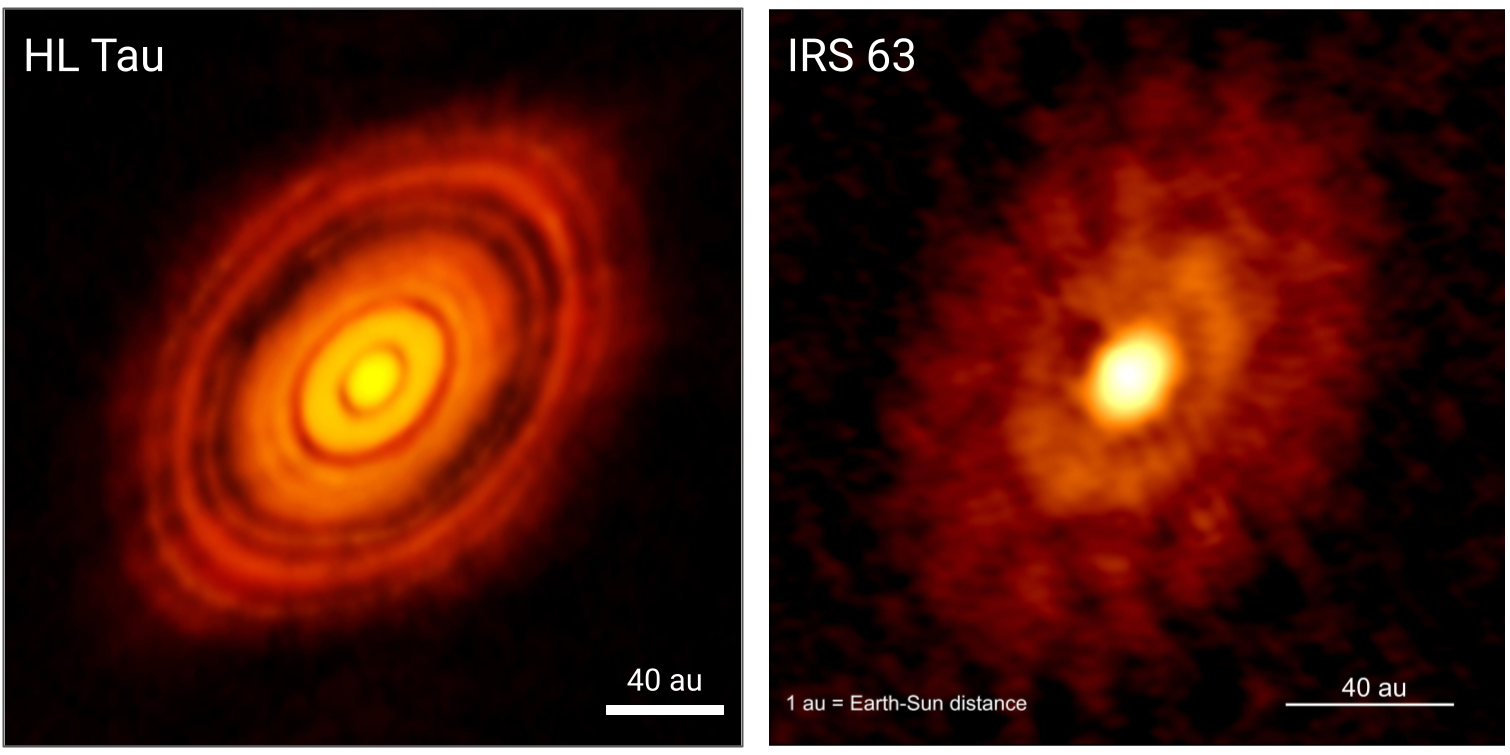
\includegraphics[width=0.99\textwidth]{WRITEUP_AND_IMAGES/IMAGES/WRITEUP/NOTMINE/IRS63_vs_HLTau_scalebar.png}
  \caption[Comparison in structure for IRS 63 and HL Tau.]{Continuum emission from HL Tau (left) and IRS 63 (right), both shown at a spatial resolution of 5 au. Scale bars represent 40 au. The HL Tau image is credited to ALMA (ESO/NAOJ/NRAO). The IRS 63 image is reproduced with permission from \cite{Dom2020}.} 
  \label{fig: HLTauIRS63}
\end{figure}  
  %\cite{ALMAPartnership} 
% Image now from 
% https://www.eso.org/public/images/eso1436a/
% https://www.eso.org/public/images/eso1436a/
% ----------------------------------------------
% --------------------------------------------------------------------
% --------------------------------------------------------------------



% --------------------------------------------------------------------
\subsection{Grain Size}
% ----------------------------------------------------
% ------------------------------------------------------------------
Previous studies of other disks have also found a similar maximum grain size using various types of observations. A well-studied disk example is HL Tau. \cite{Kataoka2016} constrained the dust grain size using polarization observations at \bsixNS, and found a maximum grain size of $\sim$ 150 \micronNS. 
This work was extended by \cite{Yang2016} to include the polarization induced by the inclination of the disk with respect to the line of sight, and found a value of 72 \micronNS. 



More recently, \cite{Mori} used multi-wavelength polarization observations between 0.87 mm and 3.1 mm to find a maximum grain size of $\sim$130 \micron and \cite{Ueda} found a similar size from polarization data of $\sim$100 \micronNS.  In comparison, \cite{Carrasco} studied HL Tau using multi-wavelength thermal emission (no polarization) with radiative transfer models and found particles on the order of a few millimetres in the central region.  Their approach also modelled dust grain sizes across HL Tau, and they found that the grain size decreased with radius to a maximum of 1 mm at 100 au.  This discrepancy in grain size with method is an open question, and suggests that either the radiative transfer models or the polarization models are sensitive to different dust regimes or are missing important physics.







Similar grain sizes have been found in other disks at different evolutionary phases, with some studies finding larger grain sizes from continuum emission than from polarization.  \cite{Ohashi} studied the protoplanetary disk IRS 48, also in the Ophiuchus molecular cloud, using ALMA polarization observations at 0.86 mm with VLA continuum observations at 8.8 mm. Their radiative transfer modelling found that in the optically thick regions of the disk the maximum grain size is likely to be $\sim$100 \micronNS. \cite{Bacciotti_2018} used ALMA polarization observations at 0.87 mm to constrain the maximum dust grain size in two Class II disks, finding 100-150 \micron for CW Tau and 50-70 \micron for DG Tau. \cite{Hu} modelled multi-wavelength continuum observations of 212 from ALMA and VLA, ranging from 0.4 mm to 3 cm, and found a maximum grain size of $\sim$130 \micronNS. More recently, \cite{Lee_2021} studied the same disk with polarization observations at 0.878 mm and found maximum grain sizes of 50-75 \micronNS.


Overall, these studies show that the maximum grain size constrained in a study can vary depending on the method and observations used, as well as location within the disk. Specifically, when a single disk is studied using multiple methods, the grain size constrained from thermal emission or spectral energy distributions tends to be larger than those constrained from polarization observations. The maximum grain sizes constrained for IRS 63 in the project, \sbest and \ibest for spherical and irregular grain models respectively, are larger than what has been found for other disks via polarization methods, including HL Tau. There has been a multi-wavelength continuum study of IRS~63 \citep{Maureira2026}, but it did not constrain the dust grain size. 


% ------------------------------------------------------------------




% --------------------------------------------------------------------
\subsection{Optical Depth}
% --------------------------------------------------------------------
% You also want to comment on the opacity and grain size of HL Tau.  You can use Carrasco-Gonzalez et al. (2019) for a dust model of HL Tau (it is generally considered optically thick throughout the disk at short wavelengths).


% Basically, in this commentary comparison, you want to make clear opacity expectations for HL Tau (from models) and what you see for IRS 63 based on where you find scattering to be significant.  The IRS 63 polarization results would suggest that it is more optically thick at its center at longer wavelengths than HL Tau. 

Another factor that can affect the dominant polarization mechanism is the optical depth of the disk. In addition to the variations in optical depth caused by the disk substructure (e.g. gaps and rings), the optical depth is also expected to change spatially across a disk, with the outer regions being more optically thin and the central regions more optically thick. Since dust self-scattering is favoured in areas with high optical depth, the consistent central region of uniform polarization in the centre of IRS~63 (Figure \ref{fig: StokesI_POLI_grid}) suggests that this region is optically thick. 


The optical depth in a disk is also wavelength-dependent and is expected to decrease with wavelength. Radiative transfer modelling of HL Tau in \cite{Carrasco} shows this relation, with the optical depth increasing at shorter wavelengths. This is consistent with the polarization morphology becoming more consistent with dust self-scattering at shorter wavelengths, as shown in Figure \ref{fig: HLTauLin2024}.


This wavelength dependence of polarization morphology provides an explanation for the same general change in morphology with wavelength seen in both HL Tau and IRS 63. Additionally, it could provide some insight into the differences in morphology between the two disks as well. Since scattering is favoured in regions with high optical depth, and dust self-scattering dominates in the central region of IRS 63 and not HL Tau, this suggests that the centre of IRS 63 could be more optically thick. The differences in optical thickness could therefore contribute to the similarity and differences between the morphologies observed in HL Tau and IRS 63. 


% --------------------------------------------------------------------


% ------------------------------------------------------------------




% ------------------------------------------------------------------
\section{Dust Properties from Scattering Models}
% ------------------------------------------------------------------

% ------------------------------------------------------------------

The scattering models for spherical grains at various porosities showed that compact ($f = 1$) and very porous grains ($f = 0.01$) provide significantly poorer fits to the observations compared to the intermediate filling factors. The goodness-of-fit improves as the filling factor decreases from $f = 1$ toward $f = 0.5$, reaches a minimum at $f = 0.5$, and then worsens towards $f = 0.01$. This preference for a porous grain indicates that the scattering properties required to reproduce the observations are best represented by porous grains, rather than a fully compact or very porous grain. This trend was seen in all fitting cases, suggesting the preferred porosity does not depend on which wavelengths are included in the fit. 
% ------------------------------------------------------------------




% ------------------------------------------------------------------
The maximum grain size also varies with filling factor. As the filling factor decreases, the best-fit maximum grain size must increase to account for the lower density in a porous grain. The irregular grain models, where porosity is not considered, have a much smaller range of best-fit grain sizes across the fitting cases. The best-fit maximum dust grain size is \sbest for spherical grains with $f=0.5$, and \ibest for irregular grains.
% ------------------------------------------------------------------


% ------------------------------------------------------------------
The spherical and irregular grain models allow us to determine the role of grain shape in polarized scattering. The lowest goodness-of-fit parameter $\chi_\mathcal{P}^2$ for spherical and irregular grain models is 1.37 and 4.54, respectively. A lower $\chi_\mathcal{P}^2$ value indicates that the best-fit spherical model matches the observational polarization fractions better than the irregular grain model. However, this does not provide strong enough evidence to claim that IRS has spherical grains over irregular grains. For example, the compact spherical grain model fit has a much higher $\chi_\mathcal{P}^2$ value of $28.80$ compared to 4.54 for the irregular grain model. This suggests that the grain shape and porosity both influence the polarization from scattering.
% ------------------------------------------------------------------


% ------------------------------------------------------------------
%In a separate paragraph, comment on the remarkable consistency between these two very similar models.  Specifically, these are two very different approaches to modelling dust, and you find a good grain size agreement between them.  Daniel was impressed by this too, if you remember, during Discs on the Exe.  I also think it is worth mentioning that this is the first study to fit multiwavelength dust polarization using these two grain models (porous + spherical versus irregular).  You could note that the true grain population is likely a combination of porous and irregular grains, but that based on your results, maximum grain sizes of ~ 210-250 um at the center of IRS 63 are reasonable.
% ------------------------------------------------------------------

The agreement between the spherical and irregular grain models is also important to consider. These are two very different approaches to modelling dust, yet the grain sizes show good agreement between them. This is the first study to fit multi-wavelength dust polarization using these two grain models, so no direct comparison to previous studies can be made. While the exact grain shape cannot be constrained, the true grain population of IRS~63 is likely to consist of a combination of porous and spherical grains. Based on the agreement between the two models, the maximum grain sizes of $\sim$201-250 \micron at the centre of IRS~63 are reasonable. 

% ------------------------------------------------------------------








 
% ------------------------------------------------------------------
\section{Implications for Dust Evolution}
% ------------------------------------------------------------------
The best-fit maximum grain sizes of \sbest and \ibestNS, for spherical and irregular grains, respectively, are significantly larger than the grain sizes expected in the ISM and the dense cores of molecular clouds, \ism and \dccNS, respectively. This difference in size provides evidence that dust grain growth is occurring in IRS 63. 

While this result is relevant to understanding the evolutionary stage of IRS 63 itself, it also has broader implications for understanding planet formation. The results suggest that the earliest steps of planet formation, dust grain growth, are already occurring at this early evolutionary stage of a disk (Class I). This is consistent with the predictions from \cite{Dom2020} and is consistent with evidence of grain growth in disks from long-wavelength measurements with the VLA (e.g., \cite{Dom2018}). This result does not provide evidence that planets have formed in IRS~63, but rather that the beginning stages of planet formation might begin at an earlier evolutionary stage than what is currently assumed by some planet formation models. Studying these younger disks therefore provides a good opportunity to probe, and therefore understand and constrain, when these planet formation processes begin.
% ------------------------------------------------------------------
% ------------------------------------------------------------------

















% ------------------------------------------------------------------
\section{Challenges with Band 5}
\label{sec: discussion_band5_data_issues}
% ------------------------------------------------------------------
\subsection{Weighting Parameter}

% \textbf{Initial Analysis.} 
The observations at \bfive were initially imaged with \texttt{robust = 0.5}, the same as the imaging parameters for the other wavelengths. Figure \ref{fig: Band5_robust05} shows the polarization data for IRS~63 at \bfive with \texttt{robust = 0.5}. The map sensitivities for \SIns, $Q$ and $U$ are roughly 13.88, 13.70, 15.20 \ujybeam (compared to 42.14, 13.32, 15.07 \ujybeam for \texttt{robust = -1}, which are presented in this work). With the larger beam and the higher sensitivity, more of the disk is recovered in polarization, as well as several polarization vectors off the disks shown in red in Figure \ref{fig: Band5_robust05}.  We attribute those red vectors to a streamer, which we discuss further in Chapter \ref{sec: streamer}.


\begin{figure}[htbp]
  \centering
  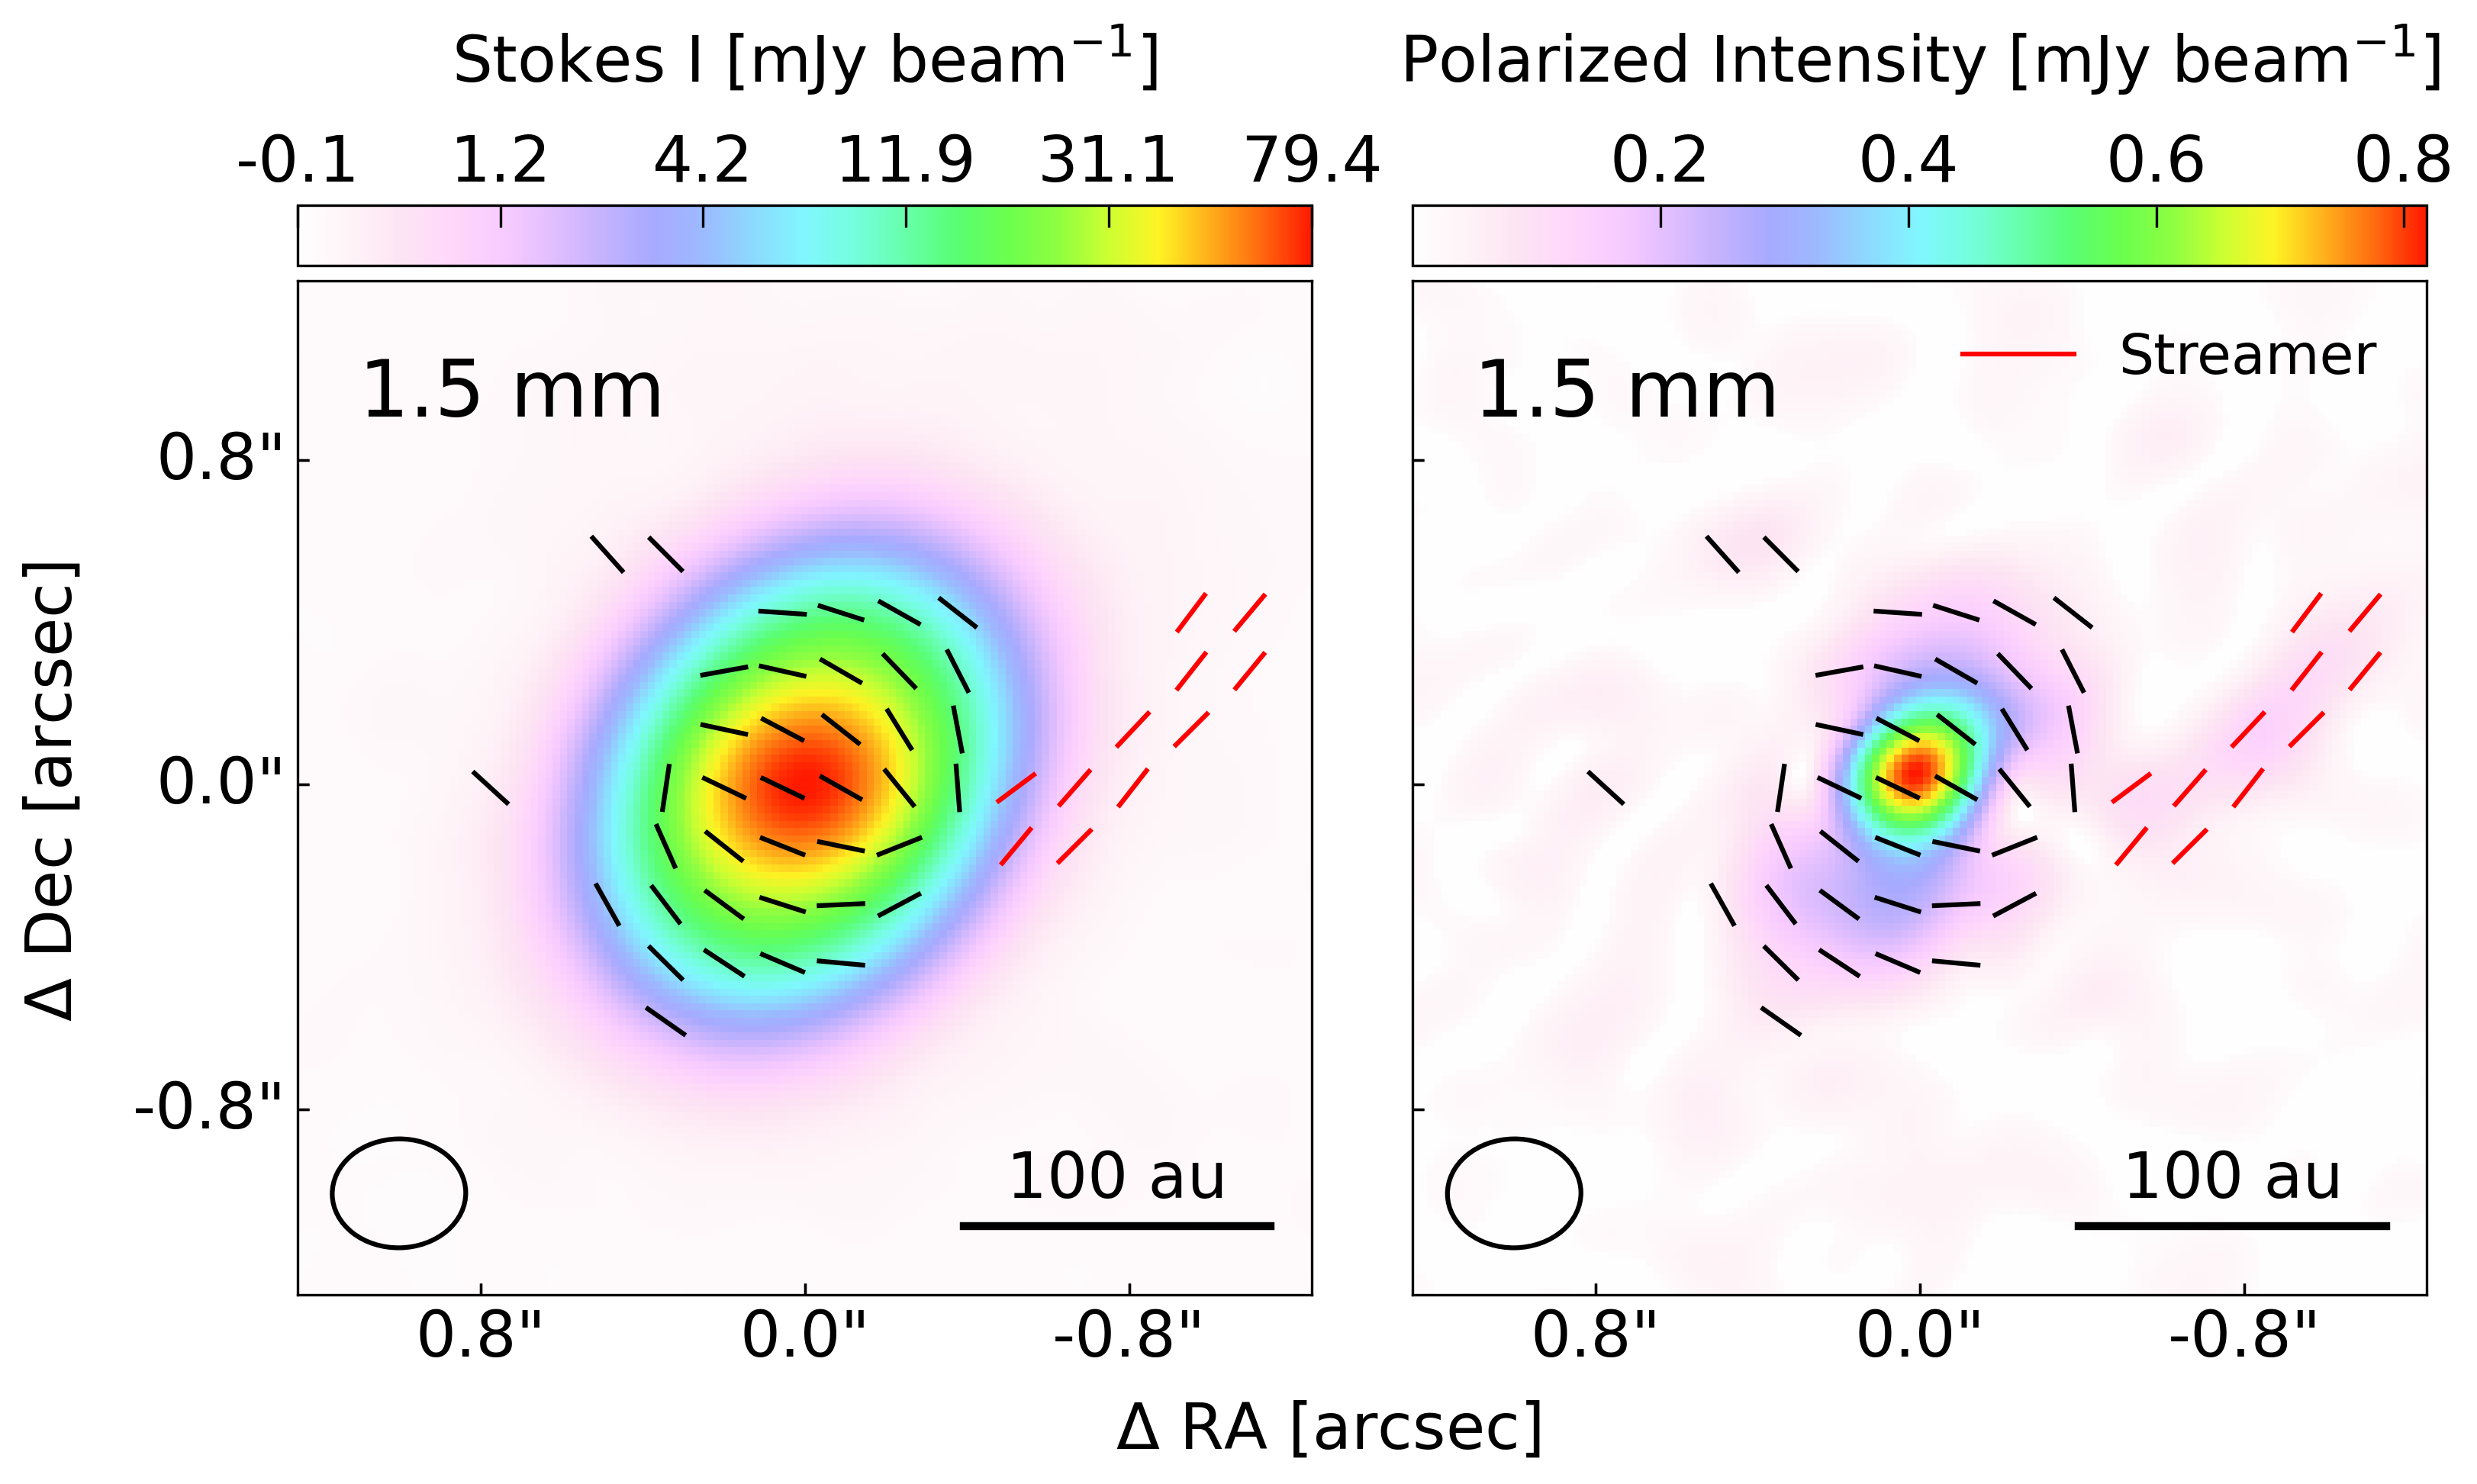
\includegraphics[width=0.75\textwidth]{WRITEUP_AND_IMAGES/IMAGES/WRITEUP/StokesI_POLI/IRS63_StokesI_POLI_vectors_BAND5_delta.png}
  \caption[Same as Figure \ref{fig: StokesI_POLI_grid} but for \bfive with \texttt{robust = 0.5}.]{Same as Figure \ref{fig: StokesI_POLI_grid} but for \bfive with \texttt{robust = 0.5}. The red vectors are for the streamer and are rotated by 90$^\circ$ to show the inferred magnetic field direction. }
  \label{fig: Band5_robust05}
\end{figure}


Nevertheless, Figure \ref{fig: Band5_robust05} shows that the central uniform region of IRS~63 is smaller than the beam resolution.  Indeed, during the dust scattering modelling for spherical grains, the \POLFsi value of 0.99 was found to be lower than expected based on the polarization fractions at the other wavelengths, and negatively affected the success of the models. Since the \bfive data have the coarsest resolution, we were motivated to determine whether or not depolarization within the beam was negatively affecting the polarization fraction at this wavelength. 










% \textbf{Imaging Differences.} 
The \rob parameter was decreased from 0.5 (\RfNS) to -1 (\RoNS), shifting the Briggs weighting closer to uniform weighting (Chapter \ref{sec: inter_weighting}). Decreasing the \texttt{robust} parameter increased angular resolution, with the beam size decreasing from $0.33'' \times 0.27''$ to $0.23'' \times 0.18''$. The higher angular resolution comes with the trade-off of lower sensitivity, with the \SIerr increasing from 14 to 42 $\mu$Jy. Due to the lower sensitivity, fewer polarization vectors are detected, and the streamer is no longer detected (Chapter \ref{sec: streamer}). 










% \textbf{Polarization Fraction and Modelling.} 
Although the polarization morphology remains similar, the \POLFsi value between the images changes. The \POLFsi value increased from 0.99 to 1.40, which agrees more with the polarization fractions measured at the other wavelengths. This shows that the choice of the \rob parameter can affect the measured polarization fraction even when the overall polarization morphology remains similar. The \Ro image and its associated polarization fraction value were therefore used for the analysis of the dust-scattering models, as its value is more consistent with the other wavelengths. Additionally, the fitting case excluding \bfive R-1 was considered to determine if it was biasing the fit. When R-1 was included, the \POLFsi was in good agreement with the model, whereas the R0.5 model did not agree. 


% ------------------------------------------------------------------

\subsection{Streamer}
\label{sec: streamer}
\label{chap: discussion_streamer}

Streamers are long, dense structures of gas acting as pathways for material to move from the surrounding envelope to the disk \citep{Heigl}. The Early Planet Formation in Embedded Disks (eDisk) study of IRS 63 first identified a candidate streamer based on observations of two molecular tracers, $^{12}$CO and C$^{18}$O \citep{Flores}. Following this, a study by \cite{Podio} presented molecular-line emission, tracing the streamer to study its impact on the southeast disk side, as shown in Figure \ref{fig: streamer}. 




\begin{figure}[htbp]
  \centering
  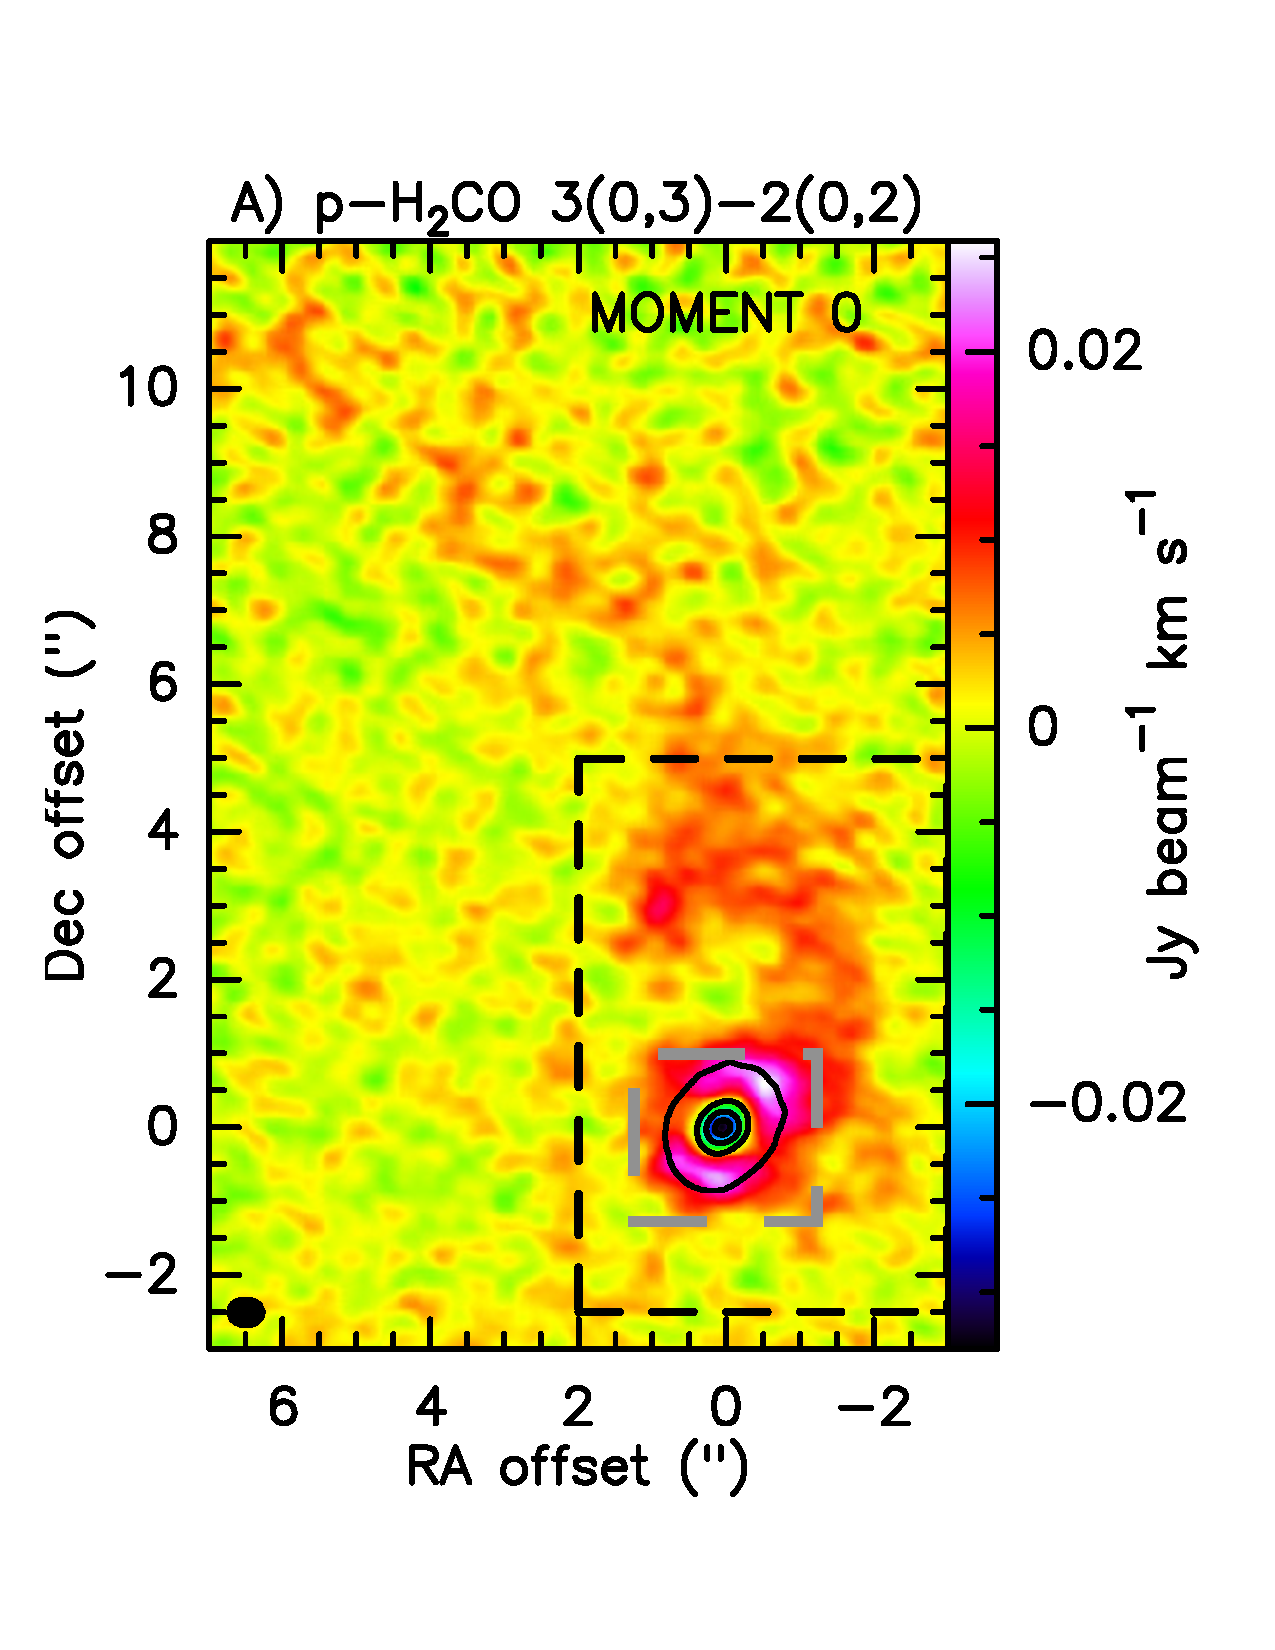
\includegraphics[width=0.5\textwidth]{WRITEUP_AND_IMAGES/IMAGES/WRITEUP/NOTMINE/aa50742-24-fig1_v2.pdf}
  \caption[Moment 0 map showing the disk and the streamer. ]{Moment 0 map of p-H$_2$CO $3(0,3)-2(0,2)$ from IRS 63, showing the disk and the streamer in the southeast region. The grey dashed box is the region shown in Figure \ref{fig: Band5_robust05}. Image from \cite{Podio}, reproduced with permission. }
  \label{fig: streamer}
\end{figure}



 During the analysis of \bfive R0.5 data, a small number of polarization vectors were found that satisfied the reliability criteria but were located outside of the disk area. These vectors are shown in red in Figure \ref{fig: Band5_robust05}, with their orientations rotated by 90\degg to show the inferred magnetic field direction, as they are likely tracing magnetically aligned grains. Additionally, the vectors have similar orientations and are detected over multiple beams, suggesting that the emission is a real feature and not due to noise. Comparing their location with the observations from \cite{Podio}, the red polarization vectors are located in the same region as the streamer. The bounds of Figure \ref{fig: Band5_robust05} are overlaid on Figure \ref{fig: streamer} as a dashed line to show the similarity between the two observations. 



The observed polarization emission in the region of the streamer is unlikely to be a result of dust self-scattering. The streamer is located outside of the dense regions of the disk, and as such, dust grains are expected to be smaller and therefore less efficient at scattering. Other polarization mechanisms cannot be ruled out. However, polarization from magnetically aligned grains is a possible explanation for the emission. If the polarization is caused by magnetic alignment, the orientation of the magnetic field can be determined since the long axes of grains tend to align perpendicular to the magnetic field \citep{Lazarian}. We note that the inferred magnetic field is aligned with the direction of the streamer, suggesting that gas flows could occur unhindered toward the disk.


Observational studies on the relationship between streamers and magnetic fields are uncommon, but some examples include SVS 13A \citep{Cort} and HOPS-182 \citep{Huang_2026}. This observation in IRS 63 may indicate a connection between the streamer and the magnetic field, providing an additional opportunity to study this relationship. However, only a few polarization vectors were detected in the streamer, and further investigation is beyond the scope of this thesis.



 

% ------------------------------------------------------------------

% ------------------------------------------------------------------





% ------------------------------------------------------------------
\section{Galaxy Contamination}




While analyzing the polarization images, we identified a faint background source at \bseven and also at \bfive (R0.5). In the \bfive data used for the majority of the analysis (R-1), the background source is not detected. Figure \ref{fig: GalaxyContamination_Both_Bands} shows the \SI images at \bfive (R0.5) and \bsevenNS, where the background source is visible slightly offset to the right of the disk, at the same position at both wavelengths. The source is not detected at \bfour and \bsixNS, likely due to a lack of sensitivity. 


\begin{figure*}[htbp]
  \centering
  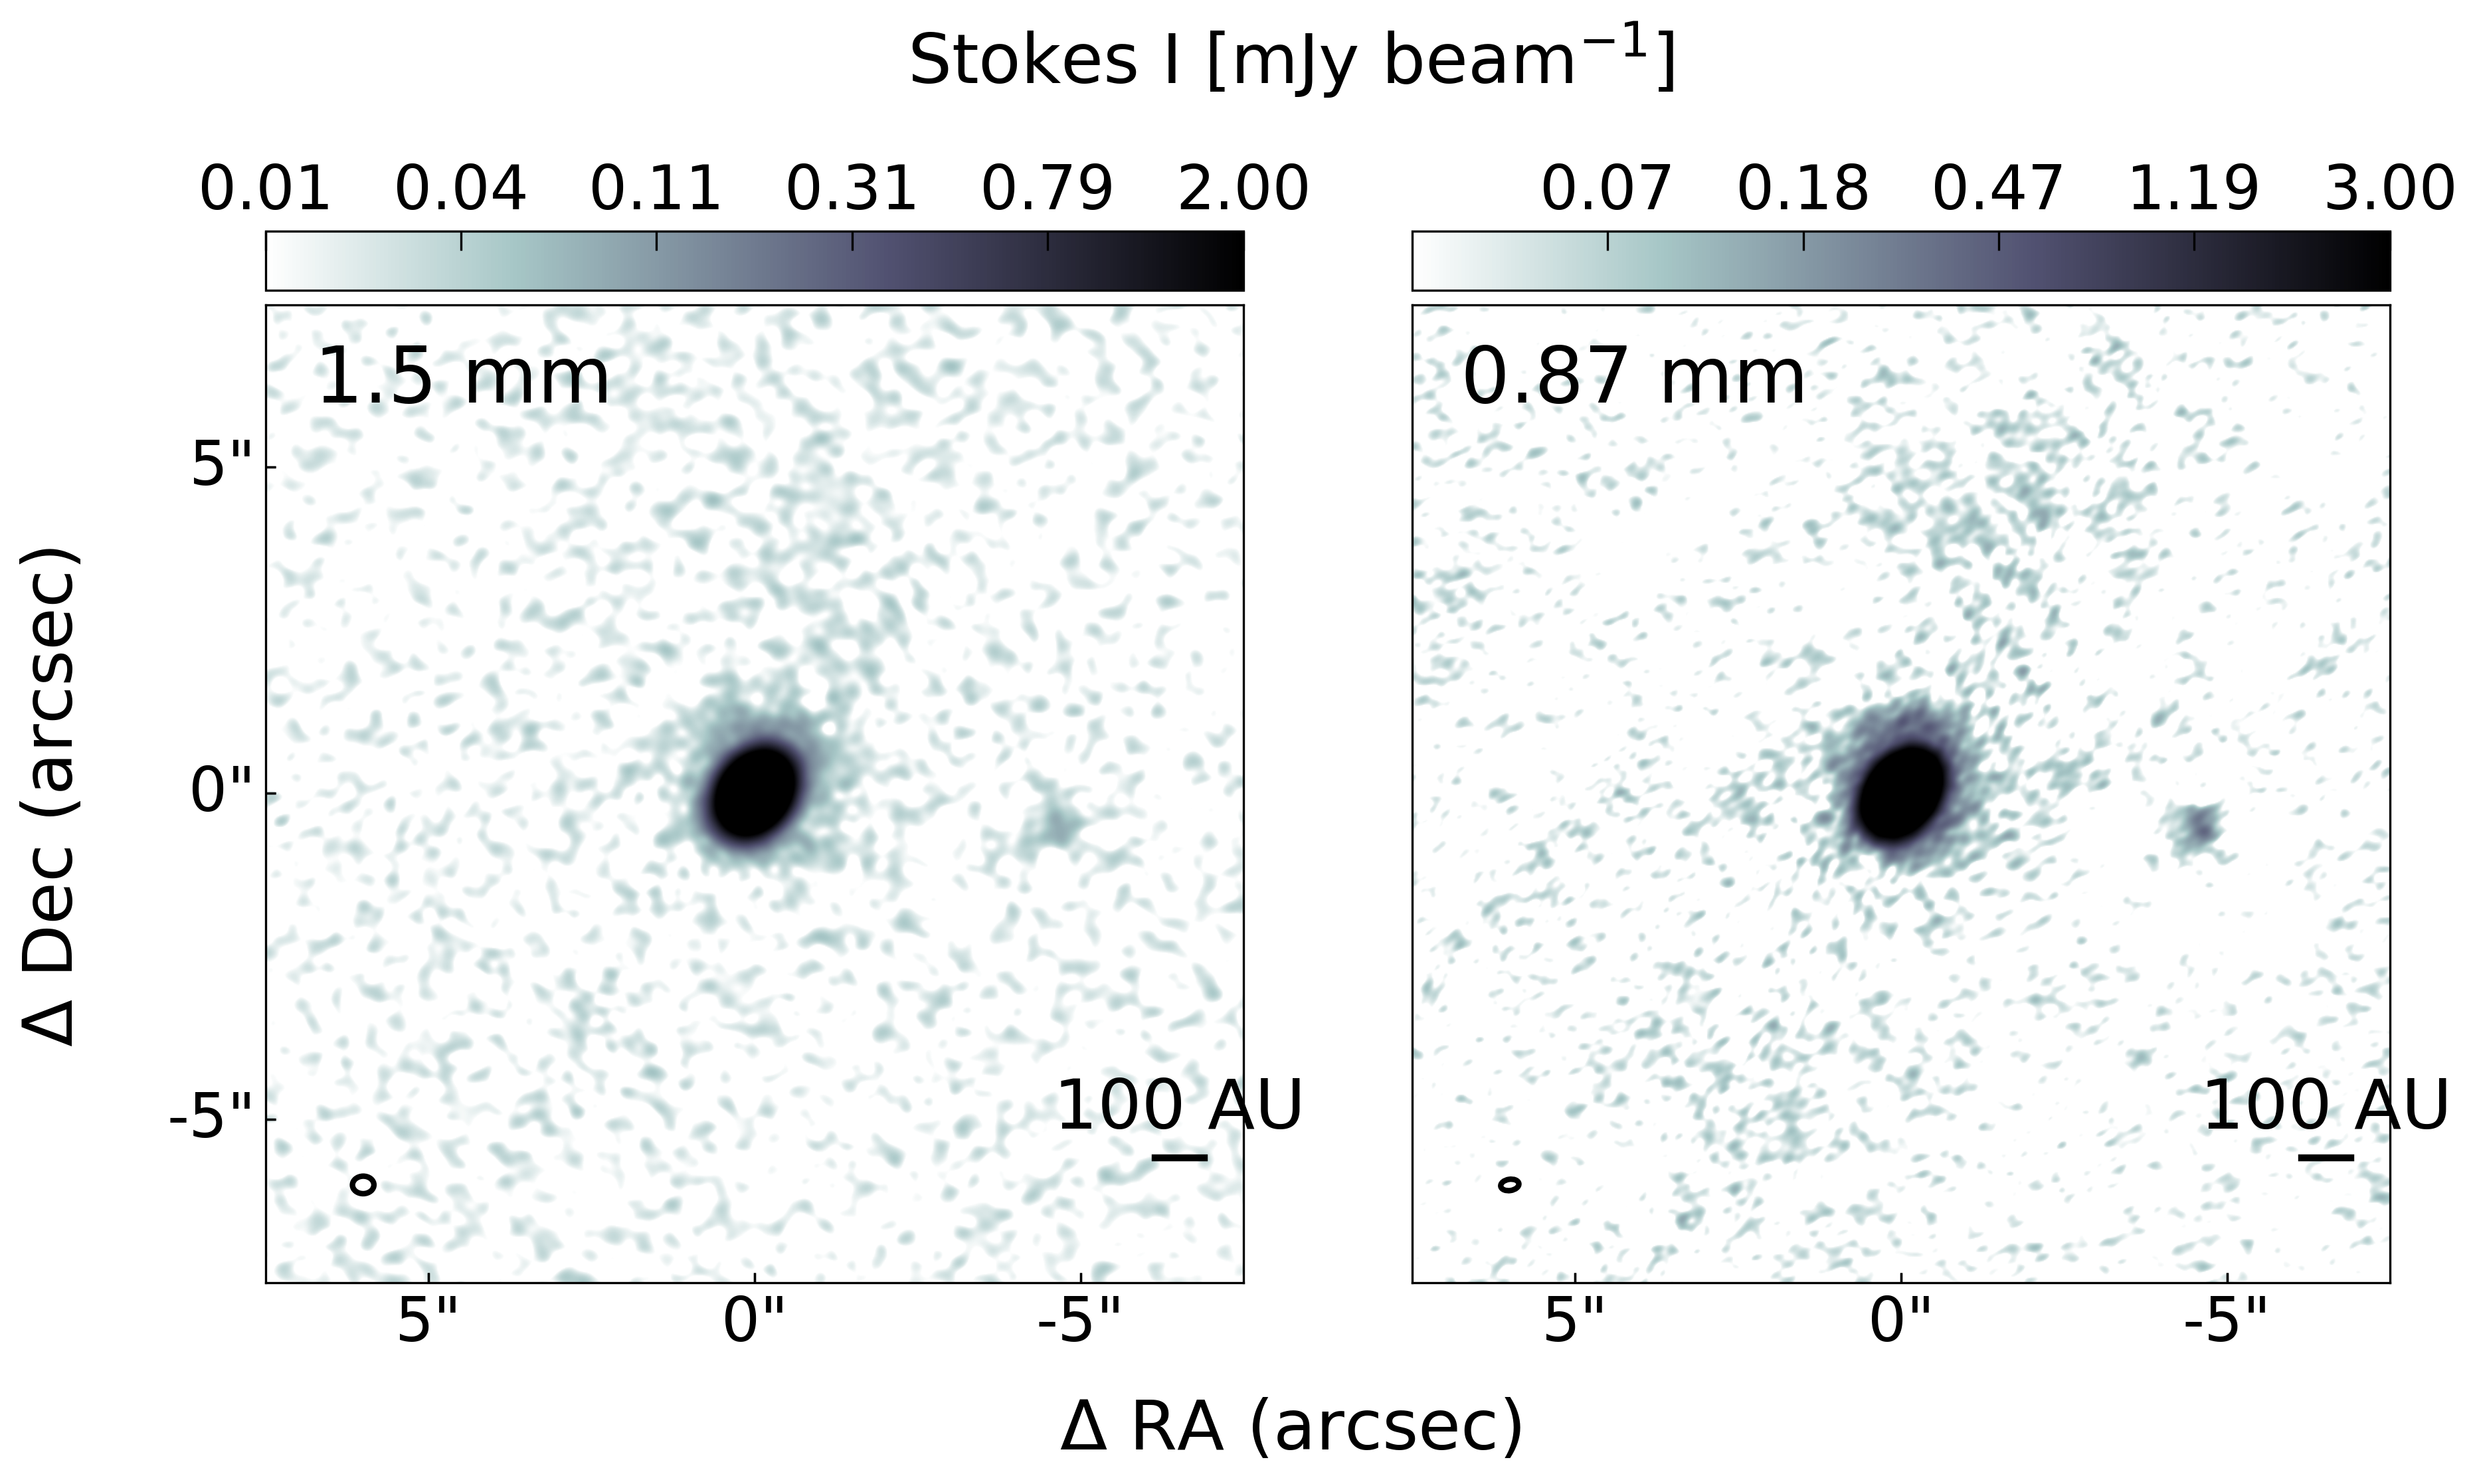
\includegraphics[width=0.75\textwidth]{WRITEUP_AND_IMAGES/IMAGES/WRITEUP/GalaxyContamination/StokesI_BothBands.png}
  \caption[\SI images showing the detected background source.]{\SI images at (left) \bfive (\texttt{robust = 0.5}) and (right) \bsevenNS, showing the detected background source. \SI values were cut off at low values to highlight the background emission.}
  \label{fig: GalaxyContamination_Both_Bands}
\end{figure*}

% \FloatBarrier

There are no known sources at the position of this object based on a SIMBAD search, suggesting that it could be a background galaxy. We estimated the probability that the source is a background galaxy following the method from \cite{sadavoy_dust_2019}. This method has also been used in other studies to estimate the number counts of background galaxies \citep{Carniani, Fujimoto}. Number counts are not well constrained at \bfiveNS, so the analysis is done only at \bsevenNS.


The galaxy number counts are described using the  Schechter function, which calculates $dN/dS$, the number of galaxies at a given flux per unit area on the sky.  The equation is given by:

\begin{equation}
\frac{dN}{dS}= N_0 \left(\frac{S}{S_0}\right)^\alpha \exp \left(- \frac{S}{S_0}\right),
\label{eq: GC_Schecter}
\end{equation}

\noindent where $N_0$ is the normalization factor, $S_0$ is the flux density at the turnover in mJy, $S$ is the intensity of the source, and $\alpha$ is the slope of the distribution \citep{Schechter}. The \bseven galaxy number counts used in the analysis were based on \cite{GC_Number_Counts}. Substituting their numbers into Equation \ref{eq: GC_Schecter} gives:
\begin{equation}
\left.\frac{dN}{dS}\right|_{0.87 \text{ mm}}
= 923\left(\frac{S}{3.9}\right)^{-1.7}
\exp\left(-\frac{S}{3.9}\right).
\label{eq: GC_Schecter_B7}
\end{equation}







To account for the changes in sensitivity across the field of view, three detection thresholds were chosen: $5\sigma(r)$, $9\sigma(r)$, and $20\sigma(r)$. Here, $\sigma(r)$ is the noise as a function of the distance from the phase centre, increasing as sensitivity decreases as you move further from the phase centre. The noise at the phase centre was chosen to be $\sigma$ = 0.035 mJy, based on the \SI uncertainty at this wavelength reported in Table~\ref{tab: source_info}. The noise as a function of radius is represented by the equation:
\begin{equation}
    \sigma(r) = \frac{0.035 \text{ mJy}}{\text{PB}(r)},
\end{equation}
\noindent where PB$(r)$ is the primary beam map.



The probability of detecting a background galaxy was calculated at concentric annuli with a radius of 0.25 arcsec. For each detection threshold, $dN/dS$ was integrated to determine the expected number of galaxies per unit area. This value was multiplied by the area of each annulus to determine the expected number of galaxies above the given threshold in each annulus, to get $N_\text{expected}$. We then converted the number of galaxies to a probability using Poisson statistics:
\begin{equation}
    \text{Probability} = 100*(1 - \exp(-N_\text{expected})).
\end{equation}


\noindent Both the probability within each annulus and the cumulative probability as a function of radius are shown in Figure \ref{fig: GalaxyContamination_Prob_B7}. 



\begin{figure}[htbp]
  \centering
  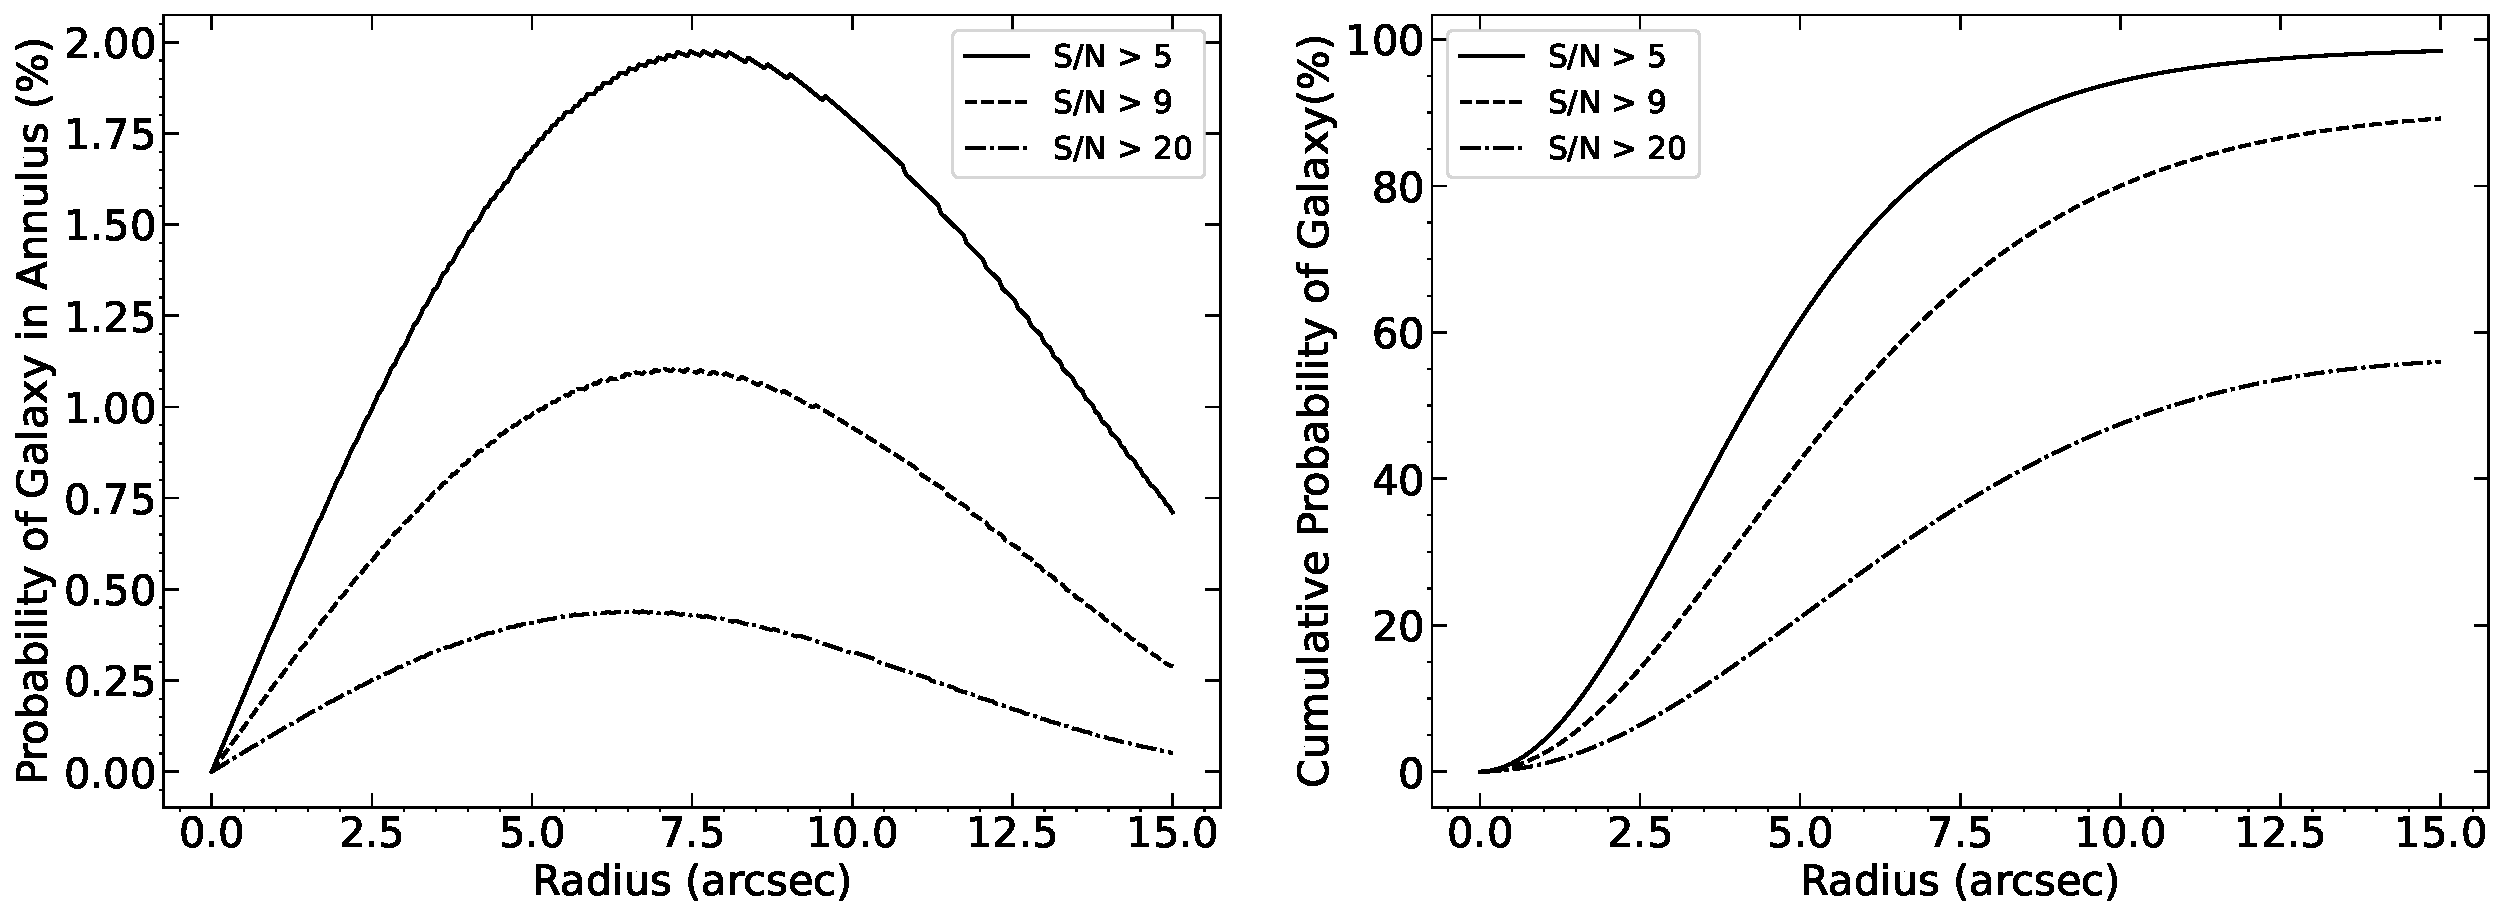
\includegraphics[width=0.99\textwidth]{WRITEUP_AND_IMAGES/IMAGES/WRITEUP/GalaxyContamination/Probabilities_Band7.pdf}
  \caption[Probability of detecting a background galaxy.]{Probability of detecting a background galaxy within an annulus (left) and cumulative probability within a given radius (right) at \bsevenNS, for detection thresholds of 5$\sigma$, 9$\sigma$ and 20$\sigma$. }
  \label{fig: GalaxyContamination_Prob_B7}
\end{figure}







The background source is located $\sim$ 4.75 arcsec from the centre of the disk, and it has a flux of 0.40 mJy, which is roughly an \SNR of 9.44 at its location. At this radius, the cumulative probabilities for sources with thresholds of $5\sigma(r)$, $9\sigma(r)$, and $20\sigma(r)$ are 58.49\%, 39.89\%, and 19.55\%,  respectively. Therefore, the $9\sigma(r)$ result is the best estimate of the probability. The probability of 39.89\% suggests that it is likely that the detected source is a background galaxy. We note, however, that the background source does not affect the main science goals of the project, as it is not a part of IRS 63.




% ------------------------------------------------------------------
\section{Limitations}
% ------------------------------------------------------------------
\subsection{Model Assumptions}

% Porosity
The dust self-scattering models have many inherent assumptions that provide limitations on the constraints that can be placed in this study. However, these assumptions also provide opportunities for future studies. 


A limitation of the models is that the porosity cannot be varied for the irregular grains. This limits the constraints we can place on grain shape and porosity of the grains, as only compact grains can be compared with both the spherical and irregular models. The agglomerated debris particles used by \texttt{glitterin} do not account for porosity in their construction \citep{glitterin}.  Future work that includes such details in the neural network would be needed.


% Composition
Another limitation that is easier to address is the composition of the grains. Currently, only DSHARP dust composition is considered. However, both \texttt{glitterin} and \texttt{DSHARP} allow the composition of the grains to be changed easily, making this an easy parameter to further study. For better comparisons with other work that used DSHARP dust compositions (e.g., \cite{Mori}, \cite{Ueda}), we focus only on the DSHARP dust here.








% Flaring 
The intensity profiles studied in Chapter \ref{sec: ch4_intensity_profiles} suggest that IRS 63 is flared, however, the models do not currently account for this disk feature. Incorporating a flared disk into the model would provide a more realistic model of the disk and could be used to determine if the scale height of the disk affects polarization.  




% Centre of the disk
The scattering models are also limited to the very centre of the disk, where dust self-scattering is observed at each wavelength. As a result, the polarized fraction value used in comparison to the models is measured at a single location rather than varying across the disk. Because of this, the scattering models do not test for any potential spatial dependence. Additionally, from the findings in \cite{Dom2020}, we know that IRS~63 is structured. An improved model that encompasses the full extent of the disk would need to also take the rings in IRS~63 into account. 



\subsection{Observational Limitations}


One observational limitation of the study is the number of wavelengths of data available. While four wavelengths is an improvement compared to single-wavelength polarization studies of IRS 63, a wider range of polarization observations would allow the transition in polarization morphology to be constrained better. Specifically, observations at shorter and longer wavelengths allow the polarization morphologies to be studied across a wider wavelength range. Additionally, stronger constraints can be placed on the scattering models as the number of observational polarization fraction values, and therefore polarization curves, can be tested. 




Higher resolution data also provides the opportunity to improve the constraints on dust grain properties. For example, \cite{Stephens2023}, used high-resolution polarization data of HL Tau, which revealed changes in the polarization morphology across the disk as the optical depth changes (e.g., due to rings and gaps). However, increasing the resolution requires longer integration times on source, which are expensive.  To date, only one disk has high-resolution ($\sim$5 au) polarization measurements (HL Tau; \cite{Stephens2023}), and such data took almost 19 hours of ALMA observing time. Therefore, as the capabilities of ALMA improve to higher resolution, future polarization observations of IRS 63 may be taken.

Additionally, simultaneously using polarization emission with other types of data could be useful. For example, models of IRS~63 in thermal dust emission that use radiative transfer can also constrain the grain size (e.g. following the approach of \cite{Carrasco}).  Such analysis would be useful to determine whether or not IRS 63 follows the same trend seen in other disks, such that thermal emission tends to infer larger grains compared to polarization observations. This would also provide the opportunity to improve the modelling of the disk, so that polarization from scattering could be studied beyond the centre of the disk. Specifically, this would involve incorporating radiative transfer equations to study the spatial dependence of the polarization morphology across the disk as a function of parameters such as optical depth.

%%% Azimuthal polarization



\subsection{Combined Polarization Modelling}
Lastly, the models for this study are currently limited to the central region of IRS~63, where the morphology indicates that dust self-scattering is dominant. An important next step would be to extend the models to the outer regions of the disk and simultaneously fit the regions with scattering and azimuthal alignment, and most importantly, their transition regions. This would allow the contributions of each mechanism to be better constrained across the disk, and could potentially characterize the \bfive R0.5 data, where scattering alone could not reproduce the observed polarization at this weighting. 


% Fold this into the scattering vs aligned part 
Extending the analysis to the outer region of the disk would also provide an opportunity to further constrain the dust grain properties. \cite{Lin2024} showed that using polarization from the outer region of the disk can be used to constrain the grain shape, specifically whether grains are prolate or oblate. Applying a similar analysis to IRS~63 could therefore provide better constraints on the grain shape and how the sizes vary across the disk. 






% \subsection{The Future of ALMA}

% Looking further into the future of ALMA, it is expected to provide new opportunities for future polarization studies of disks. While polarization studies are becoming increasingly more common, obtaining the data necessary to constrain the grain size is difficult due to long observation times and limited available hours. Theoretical developments for ALMA 2040 include increasing the number of dishes to 255 and simultaneous coverage across multiple wavelengths of data. These upgrades would significantly reduce the collection time, making a large-scale polarization population study possible. This would allow us to study how the maximum dust grain size changes with disk properties (e.g. evolutionary stage, inclination, location) and provide an opportunity to constrain when planet formation begins on a much wider scale compared to on a disk-by-disk basis.
% \noindent \note{This was just an idea based on your ALMA2040 white paper; I am not sure if (1) this is good to include, (2) something I am allowed to include since the paper is not out yet. I assume I could cite it as in prep?}
% ------------------------------------------------------------------


